\section{Validaci\'on}

El modelo propuesto para recuperar la ecuaci\'on de M\'arkus y H\'azi fue probado mediante la realizaci\'on de una serie de experimentos num\'ericos, destinados a evaluar la capacidad y precisi\'on para simular problemas de flujo multif\'asico con transferencia de calor y cambio de fase. En primer lugar, se obtuvieron soluciones num\'ericas para dos situaciones en las que es posible encontrar una soluci\'on anal\'itica: la estratificaci\'on de un fluido van der Waals en una cavidad con temperatura no uniforme, y la simulaci\'on de un frente de evaporaci\'on. Por otro lado, se simul\'o la generaci\'on de burbujas sobre una placa horizonal calefaccionada, tambi\'en conocido como ebullici\'on heterog\'enea, y se emple\'o este problema para discutir aspectos fundamentales de una simulaci\'on con lattice Boltzmann, como resoluci\'on de grilla y selecci\'on de condiciones de contorno.



\subsection{Estratificaci\'on de un fludo van der Waals}

La \eq{eq:vdw_column_red} permite describir la distribuci\'on unidimensional de densidad en un fluido van der Waals estratificado, de modo que se determina la variaci\'on de densidad en cada fase a partir de una \'unica interfase. sin embargo, a diferencia de la propuesta de Berberan-Santos \cite{berberan-santos_liquidvapor_2002}, en este caso es posible que la cavidad presente una distribuci\'onde temperatura no uniforme \cite{fogliatto_simulation_2019}. Esta flexibilidad adicional permite que este mismo problema pueda ser empleado para validar la \lbe{} propuesta. En particular, es sencillo ver que en un caso hidrost\'atico, la \eq{eq:markus_orig} puede expresarse en unidades reducidas como
\begin{equation}
	\dfrac{\partial}{\partial E_r} \left( \lambda \dfrac{\partial T_r}{\partial E_r} \right) = 0.
	\label{eq:markus_1d}
\end{equation}

Por lo tanto, para obtener una soluci\'on compatible con la \lbe{} dada por la \eq{eq:modelo_2d_full}, se completa el algoritmo descripto en la \se{sec:vdw_1d} con la incorporaci\'on de la resoluci\'on de la \eq{eq:markus_1d} usando el esquema de Patankar \cite{patankar_numerical_1980} con condiciones de temperatua fija en los extremos del dominio. De esta manera, actualizando la distribuci\'on de temperatura en el paso 4 y resolviendo de forma iterativa, es posible calcular una distribuci\'on de densidad en un dominio con una distribuci\'on de temperatura que depende del perfil de densidad final. 

Siguiendo el problema detallado en la \se{sec:vdw_1d}, se realizaron simulaciones sobre  una cavidad bidimensional con $H=300$, $L=3$ y condiciones de contorno peri\'odicas en la direcci\'on $x$. En este caso se consider\'o $E_r(H)=10^{-3}$ y una densidad inicial correspondiente al valor cr\'itico ($\rho_r = 1$) con una perturbaci\'on de $\pm 1 \%$.  Para el modelo isot\'ermico se consideraron los mismos factores de relajaci\'on y constates de simulaci\'on, con $M=1$, $G=-1$, $R=1$, $a=0.5$, $b=4$, $\tau_{\rho} = \tau_j=1$, $\tau_{e}^{-1}=\tau_{\zeta}^{-1}=\tau_{q}^{-1}=\tau_{\nu}^{-1}=1.1$, y $\sigma = 0.125$. Por otro lado, para la ecuaci\'on de energ\'ia se emplearon factores de relajaci\'on $q_i = 1$, $c_v = 4$, y par\'ametros libres de la distribuci\'on de equilibrio dados por $\alpha_1 = -1$ y $\alpha_2 = 1$. 

En una primera prueba num\'erica se fij\'o el valor de temperatura de la cara superior en $T_t = 0.99 T_c$, y se realizaron simulaciones para diferentes valores de temperatura en la cara inferior ($T_b$). Las \figs{fig:vdWColumnHT_rhor}{fig:vdWColumnHT_Tr} muestran las distribuciones de densidad y temperatura obtenidas para diferentes valores de $T_b$, donde se observa que, de forma similar a lo que ocurre con el problema isot\'ermico, la fase m\'as densa ocupa la parte inferior del dominio. Sin embargo, en este caso la distribuci\'on de temperatura final no es uniforme o fija, sino que presenta un perfil asociado a una ecuaci\'on de energ\'ia con difusividad t\'ermica constante. Esta restricci\'on determina que el perfil de $T$ presente una variaci\'on significativa en la zona de la fase de vapor, efecto que se acent\'ua con la disminuci\'on de la temperatura de la cara inferior.

La soluci\'n de este problema con lattice Boltzmann reproduce campos macrosc\'opicos con similares caracter\'isticas a los del modelo isot\'ermico, es decir, perfiles de densidad y temperatura similares a la soluci\'on anal\'itica en el seno del fluido, y con una interfase cuyo espesor disminuye con la temperatura. En este caso, la \lbe{} propuesta produce una distribuci\'on de temperatura continua a lo largo de la cavidad, mientras que el espesor no nulo de la interfase no afecta significativamente a la distribuci\'on de $T$ en la zona de la separaci\'on.

\begin{figure}[ht]
	\centering
	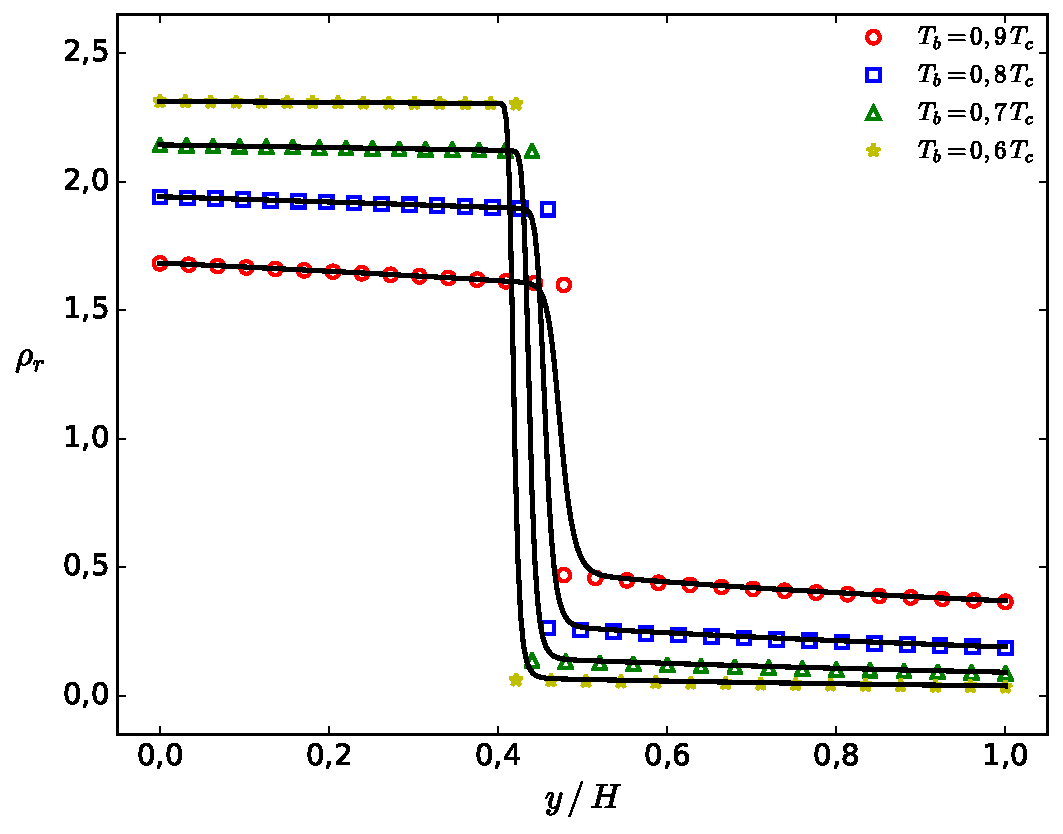
\includegraphics[width=0.75\textwidth]{vdWColumnHT_2D/CasoA/rhor_vdWcolumnHT}
	\caption{Distribuci\'on espacial de densidad en una cavidad con diferentes temperaturas en la cara inferior. Las l\'ineas continuas corresponden a simulaciones de lattice Boltzmann.}
	\label{fig:vdWColumnHT_rhor}
\end{figure}

\begin{figure}[ht]
	\centering
	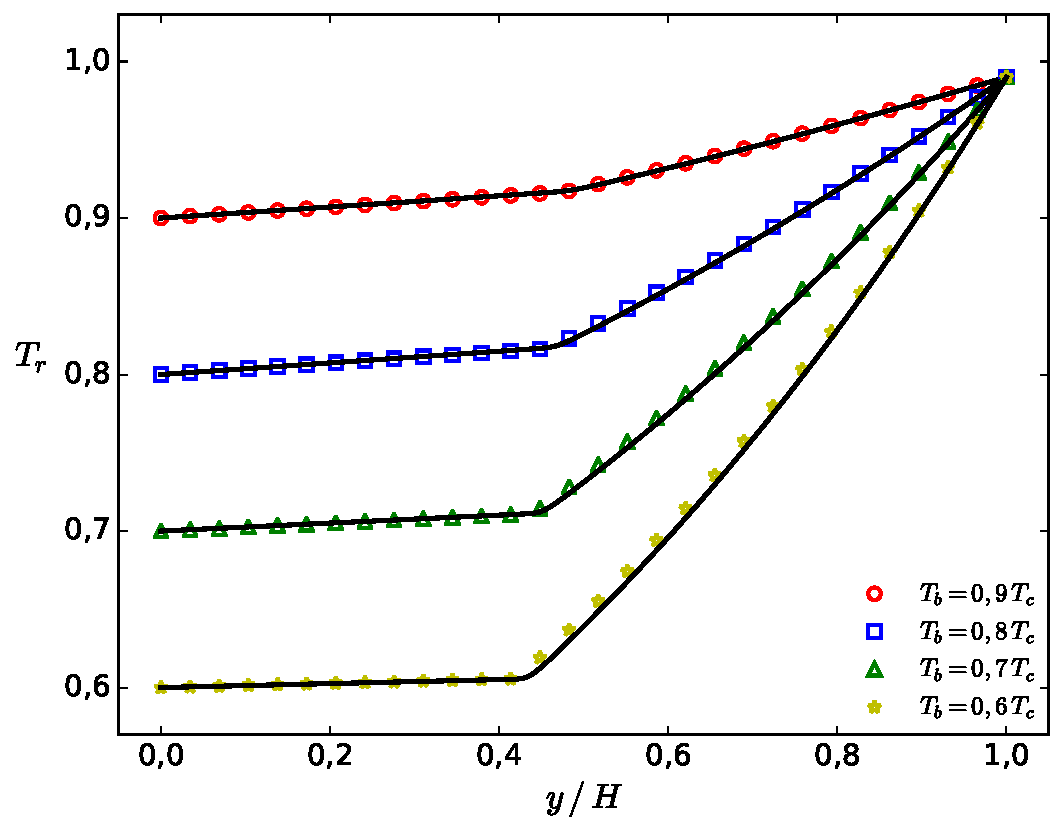
\includegraphics[width=0.75\textwidth]{vdWColumnHT_2D/CasoA/Tr_vdWcolumnHT}
	\caption{Distribuci\'on espacial de temperatura en una cavidad con diferentes temperaturas en la cara inferior. Las l\'ineas continuas corresponden a simulaciones de lattice Boltzmann.}
	\label{fig:vdWColumnHT_Tr}
\end{figure}

El problema de la cavidad constituye un excelente caso para evaluar los efectos de la resoluci\'on espacial en la reproducci\'on de la interfase. En la \fig{fig:vdWColumnHT_rhor_grilla} se muestran los perfiles de densidad reducida simulada con diferentes unidades de grilla en la direcci\'on vertical, usando $T_t = 0.99 \, T_c$ y $T_b = 0.8 \, T_c$. De forma similar a lo que ocurre con la simulaci\'on usando \'unicamente el modelo isot\'ermico, puede confirmarse que si se aplica una adimensionalizaci\'on apropiada (en variables reducidas), la concordancia entre la simulaci\'on y la soluci\'on anal\'itica mejora con el incremento de la resoluci\'on espacial. Es importante destacar que para este caso, el perfil de temperatura presenta un excelente acuerdo con la soluci\'on anal\'itica, como se muestra en la \fig{fig:vdWColumnHT_Tr}, de modo que no se observan cambios apreciables entre las diferentes resoluciones empleadas.

\begin{figure}[ht]
	\centering
	\includegraphics[width=0.75\textwidth]{vdWColumnHT_2D/CasoB/rhor_vdWcolumnHT_grilla}
	\caption{Distribuci\'on espacial de densidad en una cavidad con $T_b = 0.8 \, T_c$, $E_r(H)=10^{-3}$ y diferentes $H$. Las l\'ineas continuas corresponden a simulaciones de lattice Boltzmann.}
	\label{fig:vdWColumnHT_rhor_grilla}
\end{figure}



\begin{figure}[ht]
	\centering
	\includegraphics[width=0.75\textwidth]{vdWColumnHT_2D/CasoC/rhor_vdWcolumnHT_a_eos}
	\caption{Distribuci\'on espacial de densidad en una cavidad con $T_b = 0.8 \, T_c$, $E_r(H)=10^{-3}$ y diferentes $H$. Las l\'ineas continuas corresponden a simulaciones de lattice Boltzmann.}
	\label{fig:vdWColumnHT_rhor_grilla}
\end{figure}

\begin{figure}[ht]
	\centering
	\includegraphics[width=0.75\textwidth]{vdWColumnHT_2D/CasoD/rhor_vdWcolumnHT_b_eos}
	\caption{Distribuci\'on espacial de densidad en una cavidad con $T_b = 0.8 \, T_c$, $E_r(H)=10^{-3}$ y diferentes $H$. Las l\'ineas continuas corresponden a simulaciones de lattice Boltzmann.}
	\label{fig:vdWColumnHT_rhor_grilla}
\end{figure}